\documentclass[12pt]{article}
\usepackage[a0paper, landscape]{geometry}
\usepackage[poster]{tcolorbox}
\usepackage{anyfontsize}
\usepackage{graphicx}
\usepackage{svg}
\usepackage{xcolor}
\usepackage{optidef}
\usepackage{tikz}
\usepackage{amsmath}
\usepackage{calc}
\usepackage{adjustbox}
\usepackage[backend=biber]{biblatex}
\bibliography{references}

\usetikzlibrary{positioning, arrows.meta, calc}

\pagestyle{empty}

\definecolor{myblue}{RGB}{190, 230, 246}
\definecolor{boundark}{RGB}{18,41,93}
\definecolor{boun2}{RGB}{65,134,198}
\definecolor{green2}{RGB}{134, 198, 65}
\definecolor{darkgreen2}{RGB}{107, 158, 52}
\definecolor{pink2}{RGB}{198, 65, 134}



\begin{document}
\begin{tcbposter}[
coverage = {spread,
left=1cm,% Adjust the left margin
right=1cm,  % Adjust the right margin
top=1cm,    % Adjust the top margin
bottom=1cm, % Adjust the bottom margin
},
poster = {showframe={false},columns=4,rows=5,
},
fontsize = 36pt,
boxes = {
    titlerule=2mm,
    titlerule style={myblue,
        %arrows = {Hooks[arc=270, shorten<= 5cm]-Hooks[arc=270, shorten >= 5cm]}
        },
    arc=3mm,
    frame hidden,
    coltitle=boundark,
    colback=white,
    opacityback=0.75,
    fonttitle=\bfseries\Large,
    colupper=boundark
}
]
% Here, we insert the poster content later
\posterbox[blankest,
height=11cm,
halign=center,
valign=center,
fontupper=\bfseries,
interior engine=path,
underlay={
    \node[right,inner sep=0pt,outer sep=0pt] at (frame.west) {
\includegraphics[height=9cm]{images/boun_logo}};
    \node[left,inner sep=0pt,outer sep=0pt] at (frame.east) {
\includegraphics[height=9cm]{images/boun_logo}};
},
]
{
name=title,column=1,span=4,below=top,
}{
{\huge Partitioning Undirected Graphs}\\[8mm]
{\Large Aral Dörtoğul}\\[5mm]
{\large Advisor: Prof. Can Özturan}\\[8mm]
{\large Boğaziçi University Computer Engineering Department}
}

\posterbox[adjusted title=Problem Definition]{name=problem-definition,column=1,span=1,below=title}{
\vspace{1cm}
Partition a graph into 2 equal sized subgraphs such that the number of edges cut is minimized. Edges can have weights.
\vspace{15mm}
\begin{figure}[h]
\begin{center}
	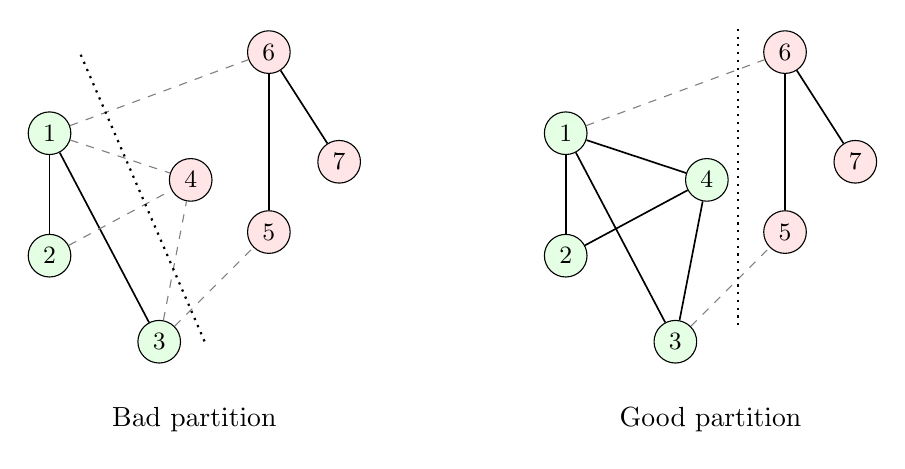
\begin{tikzpicture}[part1/.style={draw, circle, inner sep=1mm, fill=green!10},
		part2/.style={draw, circle, inner sep=1mm, fill=red!10},
		edge/.style={semithick}, cut/.style={dashed, gray}]

		\node[part1] (1-1) {\small 1};
		\node[part1, below = of 1-1] (1-2) {\small 2};
		\node[part1, below right = .7 and 1 of 1-2] (1-3) {\small 3};
		\node[part2, above right = of 1-3] (1-4) {\small 5};
		\node[part2, above right = .5 and .5 of 1-4] (1-5) {\small 7};
		\node[part2, above left = 1 and .5 of 1-5] (1-6) {\small 6};
		\node[part2, below right = 0.2 and 1.4 of 1-1] (1-7) {\small 4};

		\draw[cut] (1-1) -- (1-7);
		\draw[edge] (1-1) -- (1-2);
		\draw[edge] (1-1) -- (1-3);
		\draw[cut] (1-2) -- (1-7);
		\draw[cut] (1-3) -- (1-4);
		\draw[cut] (1-3) -- (1-7);
		\draw[edge] (1-4) -- (1-6);
		\draw[edge] (1-5) -- (1-6);
		\draw[cut] (1-1) -- (1-6);
		\coordinate[above right = .8 and .2 of 1-1] (c1);
		\coordinate[right = .3 of 1-3] (c2);

		\draw[dotted, thick] (c1) -- (c2);
		\coordinate (center1) at ($ (1-2)!.5!(1-5) $);
		\node[below = 2.4 of center1] {Bad partition};
		\node[part1,right = 6 of 1-1] (2-1) {\small 1};
		\node[part1, below = of 2-1] (2-2) {\small 2};
		\node[part1, below right = .7 and 1 of 2-2] (2-3) {\small 3};
		\node[part2, above right = of 2-3] (2-4) {\small 5};
		\node[part2, above right = .5 and .5 of 2-4] (2-5) {\small 7};
		\node[part2, above left = 1 and .5 of 2-5] (2-6) {\small 6};
		\node[part1, below right = 0.2 and 1.4 of 2-1] (2-7) {\small 4};

		\draw[edge] (2-1) -- (2-7);
		\draw[edge] (2-1) -- (2-2);
		\draw[edge] (2-1) -- (2-3);
		\draw[edge] (2-2) -- (2-7);
		\draw[cut] (2-3) -- (2-4);
		\draw[edge] (2-3) -- (2-7);
		\draw[edge] (2-4) -- (2-6);
		\draw[edge] (2-5) -- (2-6);
		\draw[cut] (2-1) -- (2-6);

		\coordinate[above left  = .1 and .4 of 2-6] (c3);
		\coordinate[below left  = 1 and .4 of 2-4] (c4);

		\draw[dotted, thick] (c3) -- (c4);
		\coordinate (center2) at ($ (2-2)!.5!(2-5) $);
		\node[below = 2.4 of center2] {Good partition};
\end{tikzpicture}
\end{center}
\caption{Different partitions of a graph}%
\label{fig:good-bad-partition}
\end{figure}

\vspace{1cm}
}
% Methodology
\posterbox[adjusted title=Methodology]
  {name=methodology, column=1, above = bottom}{
    \vspace{1cm}
    \section*{Integer Programming (IP)}

\begin{itemize}
        \item IP is an optimization method with integer-valued decision variables.
        \item Usually addresses problems involving discrete choices.
    \end{itemize}
  }
% Motivation
\posterbox[adjusted title=Motivation]{name=motivation, column=1, between=problem-definition and methodology, span=1}{
\vspace{1cm}
\begin{itemize}
    \item It is usually better to divide the data into partitions that have \textit{equal load} so that algorithms on data can be operated in a parallel fashion by multiple processors.
    \item Parallelism brings the problem of interprocessor communication, which is time consuming.
    \item It is crucial to divide the data in a way that \textit{the communication between processors is minimized}.
    \item This can be modeled as a \textbf{graph partitioning problem}.
\end{itemize}
\vspace{2cm}
\begin{center}
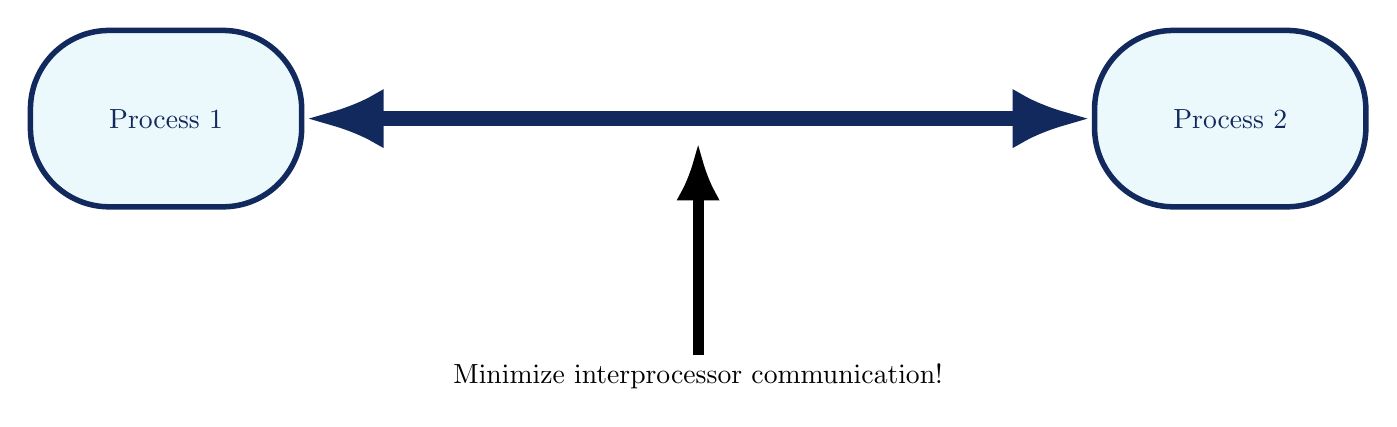
\begin{tikzpicture}
    \node[draw, color=boundark, line width=0.7mm, rounded corners=1cm, minimum width=5mm, fill=myblue!30, inner sep=10mm] (p1) {Process 1};
    \node[draw, color=boundark, line width=0.7mm, rounded corners=1cm, minimum width=5mm, fill=myblue!30, inner sep=10mm, right = 10cm of p1] (p2) {Process 2};
    \draw[Latex-Latex, line width=2mm, color=boundark] (p1) -- (p2);
    \coordinate (mid) at ($(p1)!0.5!(p2)$);
    \node[below = 3cm of mid] (text) {Minimize interprocessor communication!};
    \draw[-Latex, line width=4pt, shorten >=3mm] (text) -- (mid);
\end{tikzpicture}
\end{center}
}

\posterbox[adjusted title=References, fit,fit basedim=30pt]
  {name=references,column=2, span=2, above= bottom}{
  \printbibliography[heading=none]
}

% Methodology
\posterbox[adjusted title=How to Solve IP Models?]
  {name=ip-methods, column=2, between = title and references}{
    \vspace{1cm}
    \section{Branch and Bound}

    \begin{itemize}
        \item Tree-based recursive solution algorithm.
    \end{itemize}
    \begin{center}
\begin{adjustbox}{max width=\linewidth}
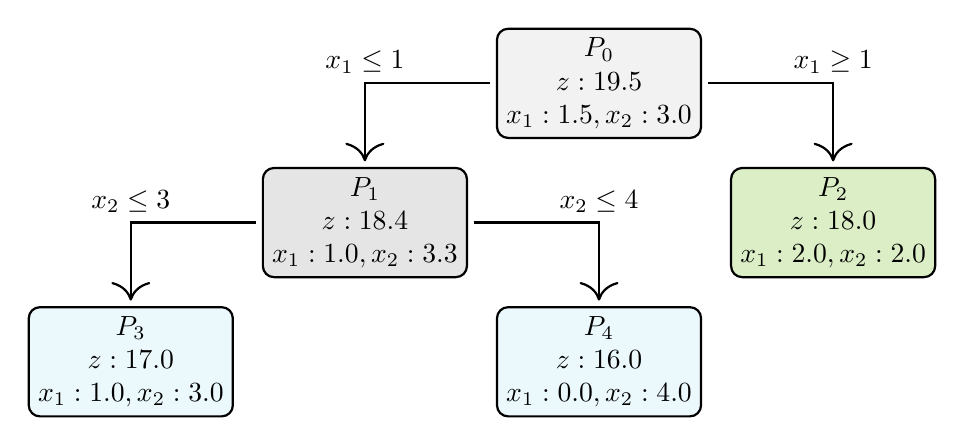
\begin{tikzpicture}[
    node/.style={draw, rectangle, rounded corners, align=center, thick},
    arrow/.style={arrows = {->[scale=2]},thick, shorten >= 2pt, shorten <= 2pt}]
\node[node, fill=gray!10] (0) {\( P_0 \)\\ \( z: 19.5 \) \\ \( x_1: 1.5,  x_2: 3.0 \) };
\node[node, below left = .5 of 0, fill=gray!20] (1) {\( P_1 \) \\ \( z: 18.4 \) \\ \( x_1: 1.0, x_2: 3.3 \)};
\node[node, below right =.5  of 0, fill=green2!30] (2) {\( P_2 \) \\ \( z: 18.0 \) \\ \( x_1: 2.0, x_2: 2.0 \)};
\node[node, below left = .5 of 1, fill=myblue!30] (3) {\( P_3 \) \\ \( z: 17.0 \) \\ \( x_1: 1.0, x_2: 3.0 \)};
\node[node, below right = .5 of 1, fill=myblue!30] (4) {\( P_4 \) \\ \( z: 16.0 \)\\ \( x_1: 0.0, x_2: 4.0 \)};

\draw[arrow] (0) -| node[midway, above] {\( x_1 \le 1 \)}(1);
\draw[arrow] (0) -| node[midway, above] {\( x_1 \ge 1 \)} (2);
\draw[arrow] (1) -| node[midway, above] {\( x_2 \le 3 \)} (3);
\draw[arrow] (1) -| node[midway, above] {\( x_2 \le 4 \)} (4);
\end{tikzpicture}
\end{adjustbox}
\vspace{5mm}

{\small Figure 2: An IP problem solved with branch~and~bound.}
\end{center}
    \section{Cutting Plane}
    \begin{itemize}
        \item Iteratively refines the feasible region.
        \begin{center}
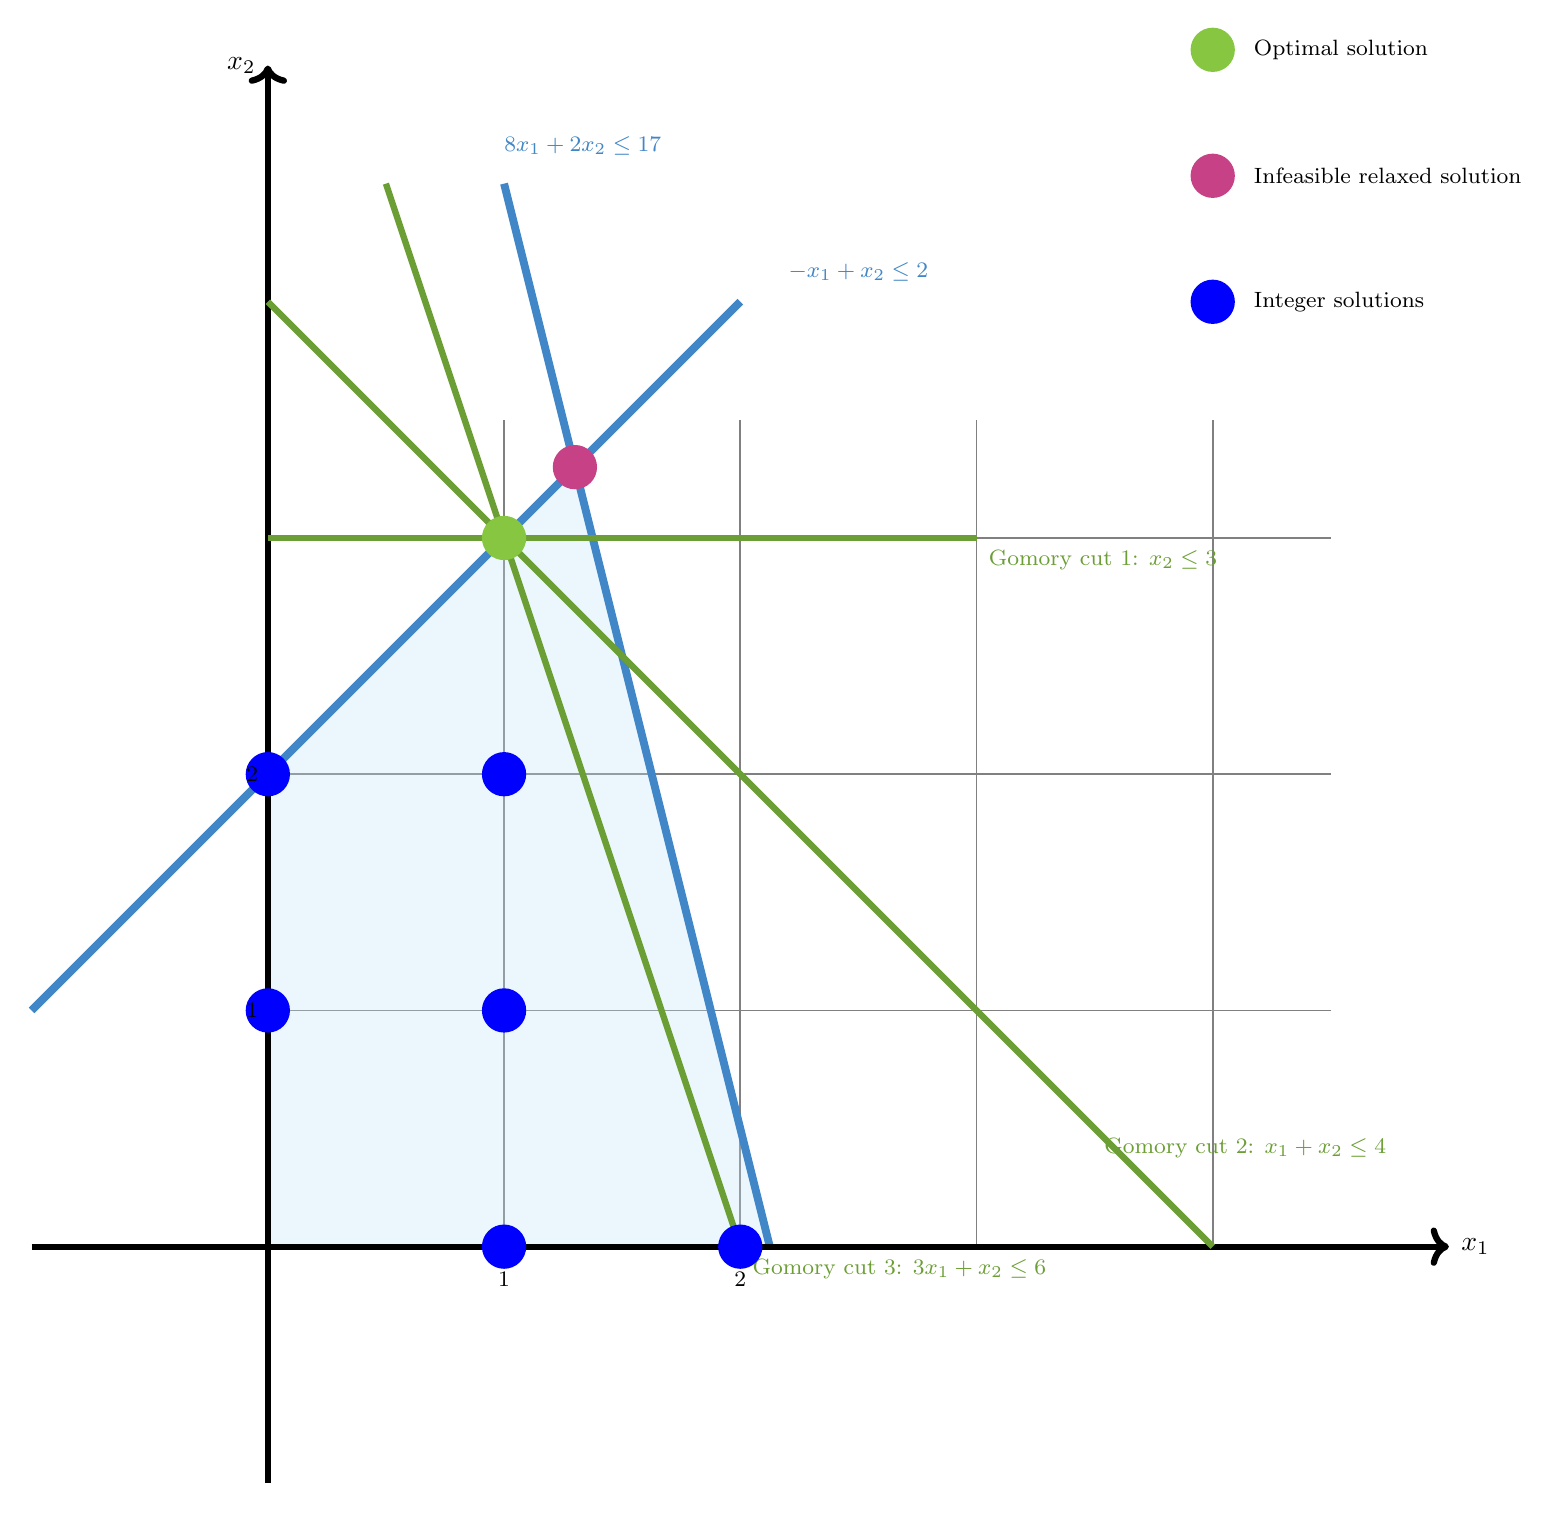
\begin{tikzpicture}[]
	\draw[step=3cm, gray, line width=0.2mm] (0,0) grid (13.5cm,10.5cm);
    \fill[myblue, opacity=0.3] (3.9cm, 9.9cm) -- (0,6cm) -- (0,0) -- (6.375cm,0cm) -- cycle;
	
	\draw[->, line width=0.8mm] (0,-3cm) -- (0,15cm) node[left] {\( x_2 \)};
	\draw[boun2, line width=1mm] (-3cm,3cm) -- (6,12) node[above right = 1mm and 15mm, anchor=south] {\footnotesize \( -x_1 + x_2 \le 2 \)};
 	\draw[boun2, line width=1mm] (6.375cm,0cm) -- (3cm,13.5cm) node [above right = 2mm and 1cm, anchor=south] {\footnotesize \( 8x_1 + 2x_2 \le 17 \)};
    \draw[->, line width=0.8mm] (-3cm,0) -- (15cm,0) node[right] {\( x_1 \)};
 
	\fill [pink2] (3.9cm, 9.9cm) circle (8pt);

	\draw[darkgreen2, line width=0.8mm] (0,9cm) -- (9cm,9cm) node [below right] {\footnotesize Gomory cut 1: \( x_2 \le 3 \)};
	\draw[darkgreen2, line width=0.8mm] (0,12cm) -- (12cm,0);
    \node at (10.5cm, 1cm) [darkgreen2, anchor=south west] {\footnotesize Gomory cut 2: \( x_1 + x_2 \le 4 \)};
	
	\draw[darkgreen2, line width=0.8mm] (1.5cm,13.5cm) -- (6cm,0) node [below right] {\footnotesize Gomory cut 3: \( 3x_1 + x_2 \le 6 \)};

        \fill[blue] (3cm,0) circle (8pt) node [below = 2mm, black] {\footnotesize 1};
        \fill[blue] (6cm,0) circle (8pt) node [below = 2mm, black] {\footnotesize 2};
    
        \fill[blue] (0, 3cm) circle (8pt) node [left, black] {\footnotesize 1};
        \fill[blue] (0, 6cm) circle (8pt) node [left, black] {\footnotesize 2};

	\foreach \position in {(3cm,3cm), (3cm,6cm)} {
		\fill[blue] \position circle (8pt);
	}
	\fill[green2] (3cm,9cm) circle (8pt);

	\fill[blue] (12cm,12cm) circle (8pt) node [right= 4mm, black] {\footnotesize Integer solutions};
	\fill [pink2] (12cm,13.6cm) circle (8pt) node [right= 4mm, black] {\footnotesize Infeasible relaxed solution};
	\fill[green2] (12cm,15.2cm) circle (8pt) node [right= 4mm, black] {\footnotesize Optimal solution};
\end{tikzpicture}

{\small Figure 3: An IP problem solved with cutting plane.}
\end{center}
    \end{itemize}
  \section{Gurobi}
    \begin{itemize}
        \item Parallel optimization solver
        \item Uses both branch \& bound and cutting plane.
        \item Efficient for linear, integer, quadratic programming.
        \item Gurobi is used in the software~\cite{dortogul}.
    \end{itemize}
  }



\posterbox[adjusted title=Integer Programming Model]
  {name=model, column=3, between=title and references}{
\vspace{1cm}
\setcounter{section}{0}
\section{Sets}
\begin{itemize}
	\item \( V = \left\{ 1,\dots,n \right\}  \): the set of vertices.
\end{itemize}

\section{Parameters}
\begin{itemize}
	\item \( w_{ij} =\) weight of edge \(i\)-\(j\),\hspace{1cm}\(\forall i,j \in V,\hspace{1cm}i<j\)
\end{itemize}

\section{Decision Variables}
\begin{itemize}
	\item \( x_{ij} = \begin{cases}
		1, &\text{edge from \( i \) to \( j \) is ``cut''}\\
		0, & \text{otherwise}
	\end{cases},\hspace{5mm}\parbox{49mm}{\centering \(\forall i,j \in V\)\\\(i<j\)\\\(w_{ij} \neq 0\)}\)
 
	\item \( p_i = \begin{cases}
		1, &\text{vertex \( i \) is in partition \#1}\\
		0, & \text{vertex \( i \) is in partition \#0}
	\end{cases},\hspace{1cm}\forall i \in V \)
\end{itemize}

\section{Objective Function}

\begin{center}

\begin{tikzpicture}
    \node[draw=boundark, rectangle, line width=0.7mm, fill= myblue!30, inner sep=12mm, minimum width=26cm, rounded corners=1cm]{\large \(\min{Z} = \displaystyle\sum_{i=1}^{n-1} \displaystyle\sum_{j\in V | i<j, w_{ij} \neq 0} w_{ij} \times x_{ij}\)};
\end{tikzpicture}
\end{center}

\section{Constraints}

\begin{enumerate}
    \item Adjacent nodes are in the same partition
    \begin{itemize}
        \item \(p_i - p_j \le x_{ij} \hspace{2cm} \forall i,j \in V,\hspace{1cm}i<j\hspace{1cm}w_{ij} \neq 0\)
        \item \(p_i - p_j \ge -  x_{ij} \hspace{1cm}\forall i,j \in V,\hspace{1cm}i<j\hspace{1cm}w_{ij} \neq 0\)
    \end{itemize}

    \item Equal partition sizes
    \begin{itemize}
        \item \(\displaystyle\sum_{i=1}^{n} p_i = \left \lfloor \frac{n}{2}  \right \rfloor\)
    \end{itemize}

    \item Binary variable constraints
    \begin{itemize}
        \item \(x_{ij} =\left\{ 0,1 \right\} \hspace{1cm}\forall i,j \in V,\hspace{1cm}i<j\hspace{1cm}w_{ij} \neq 0\)
        \item \(p_i =\left\{ 0,1 \right\} \hspace{1cm}\forall i \in V\)
    \end{itemize}
\end{enumerate}
}
\posterbox[adjusted title=Testing \& Results]
  {name=algorithm,column=4,between=title and references}{
  \vspace{1cm}
  {\small The software~\cite{dortogul} is tested on various graph sizes/densities:}
  
  \vspace{1cm}
  {\Large \textbf{Key Findings}}
  
  \begin{itemize}
      \item The software can partition graphs of any density when the graph's size is less than 50.
      \item When the graph's size is greater than 50, complexity of the problem increases very quickly and the software can only partition sparse graphs.
      \item On average, weightless version of the problem takes slightly more time to solve than the weighted version.

  \end{itemize}

  \begin{minipage}{.5\linewidth}
        \centering
        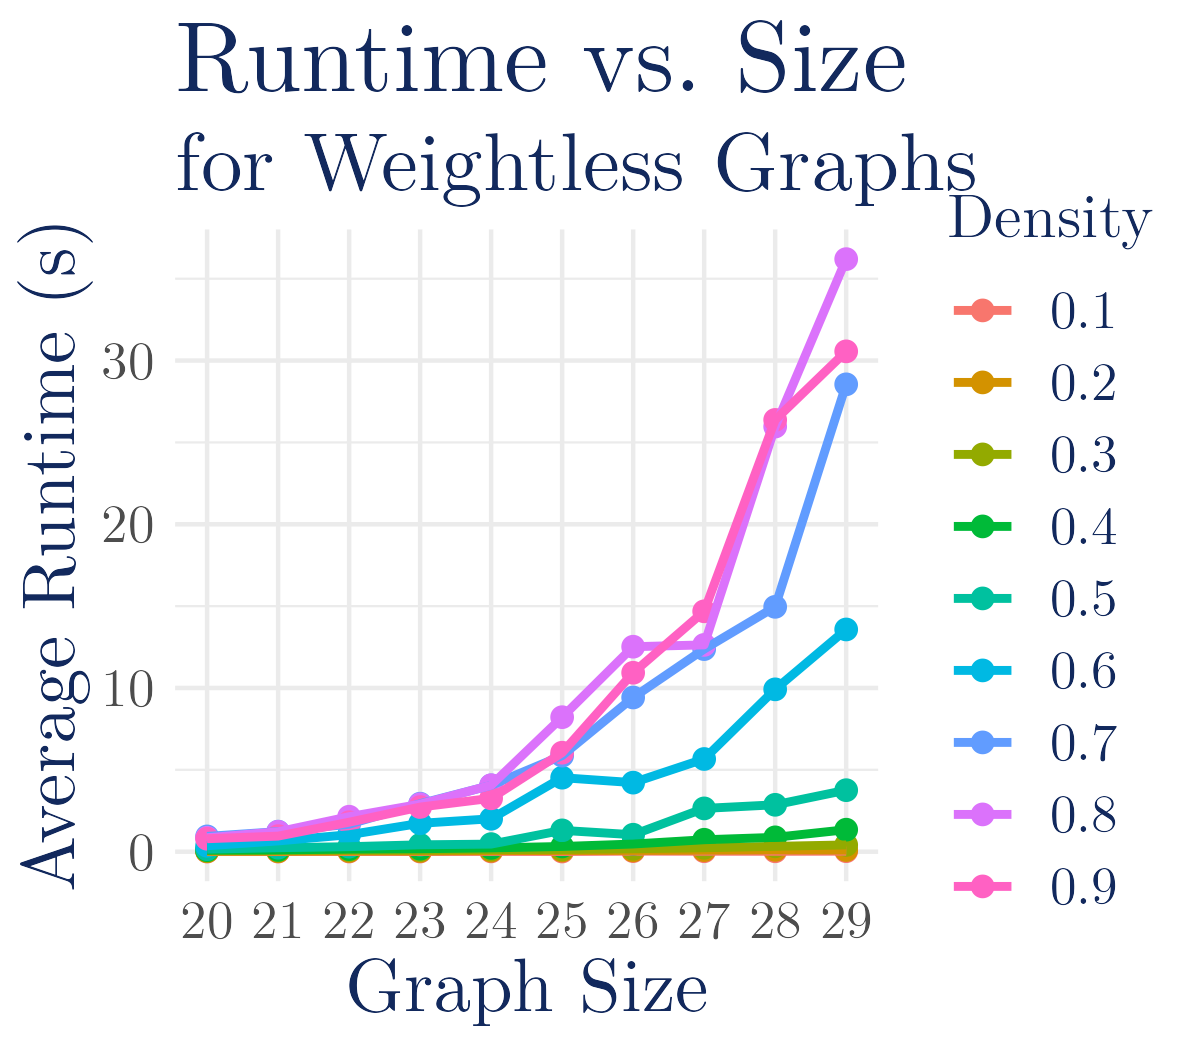
\includegraphics[width=\linewidth]{images/p1}\\
        {\footnotesize (a)}
    \end{minipage}%
    \begin{minipage}{0.5\linewidth}
        \centering
        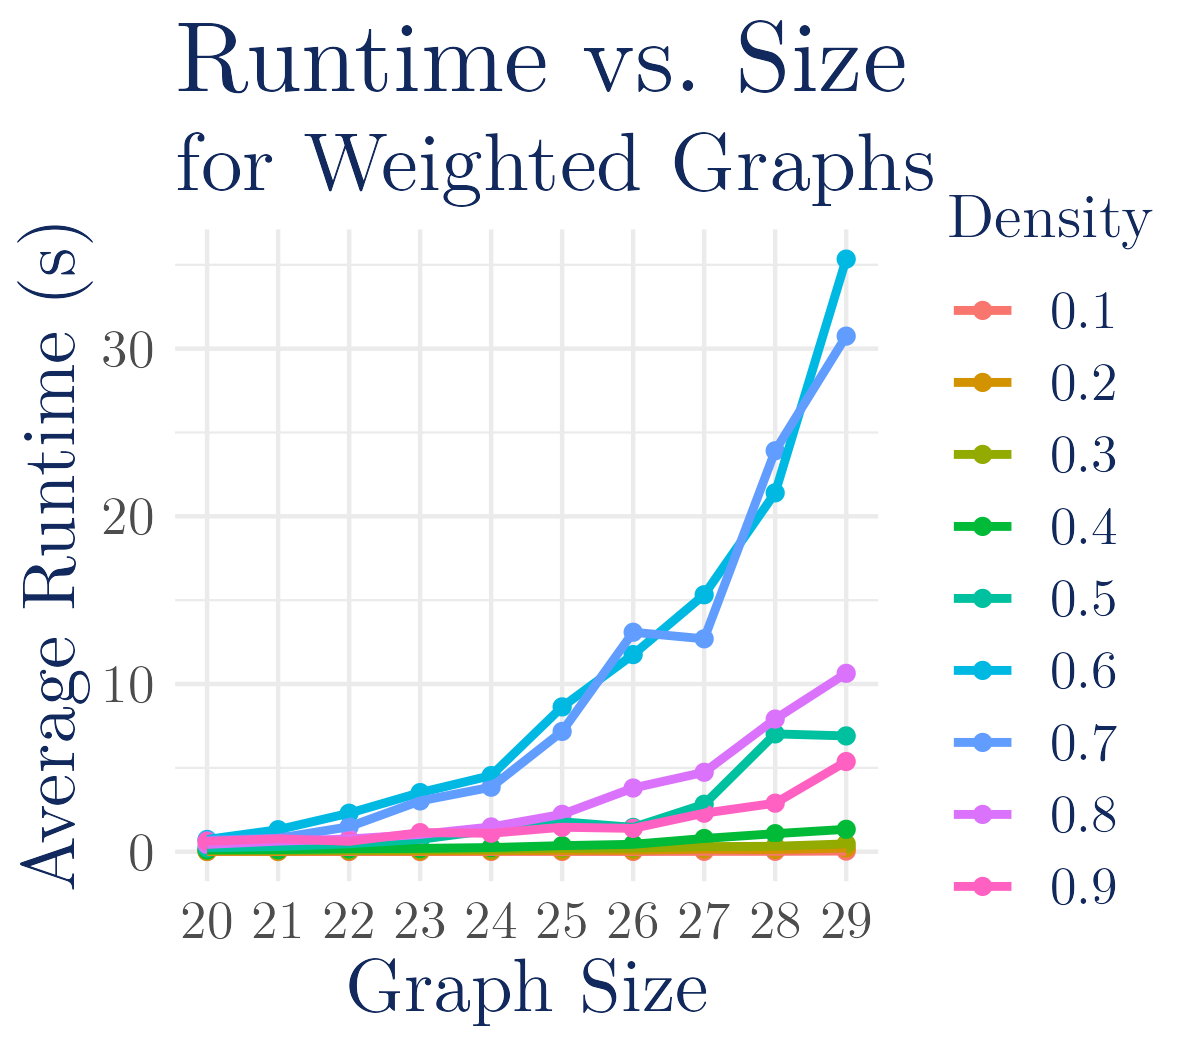
\includegraphics[width=\linewidth]{images/p2}
        {\footnotesize (b)}
    \end{minipage}
    \begin{center}
        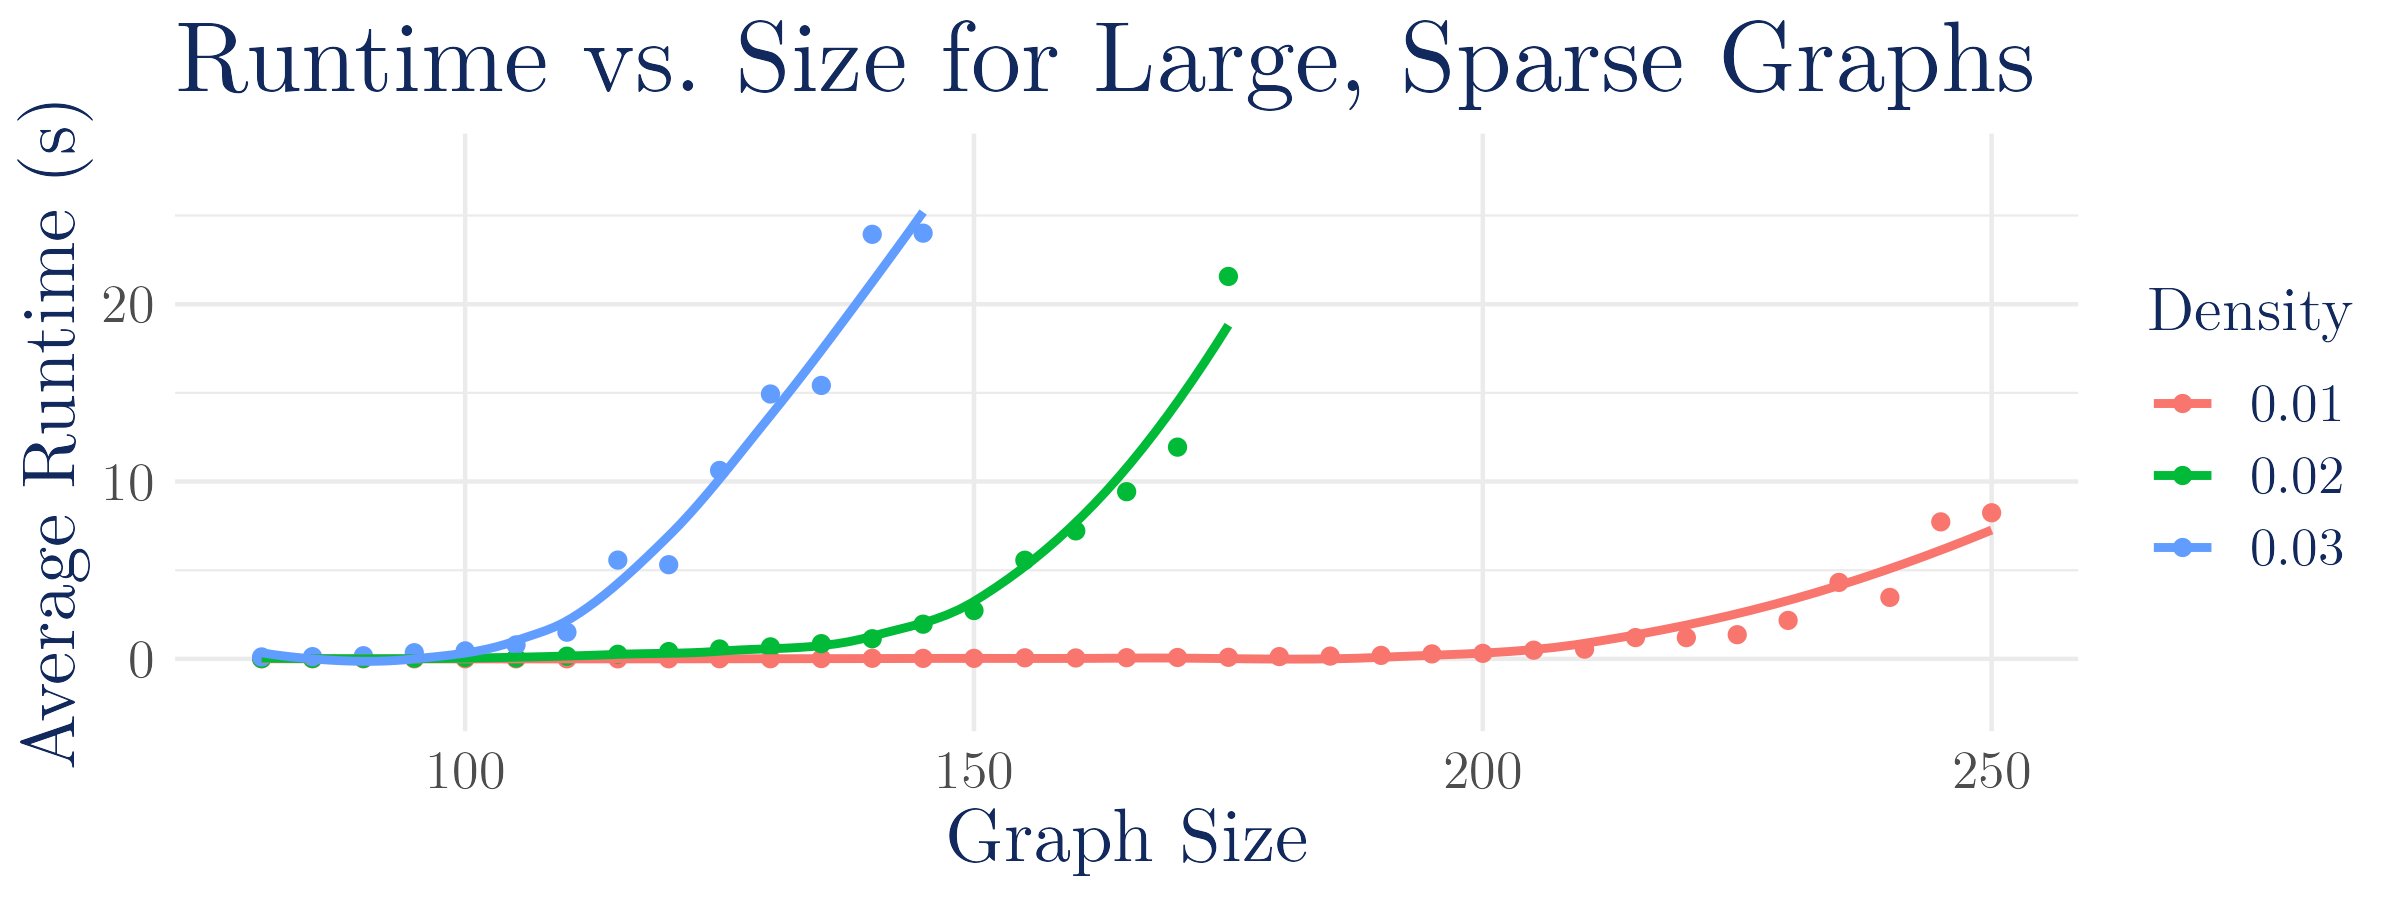
\includegraphics[width=\linewidth]{images/p3}
        {\footnotesize (c)}

        {\small Figure 4: Plots of the runtime of the algorithm}
    \end{center}
    
\vspace{1cm}
{\Large \textbf{Showcase}}

\begin{minipage}{.5\linewidth}
        \centering
        \includesvg[width=\linewidth]{images/graph20}
    \end{minipage}%
    \begin{minipage}{0.5\linewidth}
        \centering
        \includesvg[width=\linewidth]{images/graph60}
    \end{minipage}

    \begin{minipage}{.5\linewidth}
        \centering
        \includesvg[width=\linewidth]{images/wgraph20}
    \end{minipage}%
    \begin{minipage}{0.5\linewidth}
        \centering
        \includesvg[width=\linewidth]{images/wgraph60}
    \end{minipage}
    
  
}

\end{tcbposter}
\end{document}